\section{آشنایی با مشخضه i-v دیود}
\subsection{الف)}
\begin{figure}[h]
    \centering
    \fbox{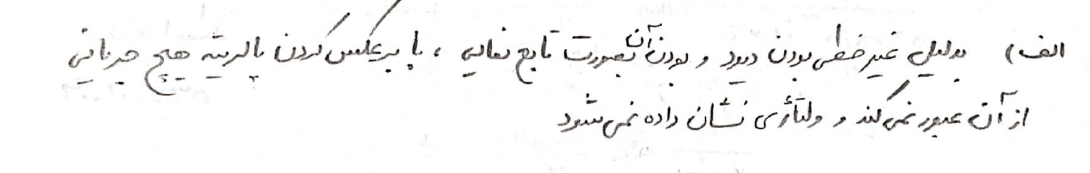
\includegraphics[width = \textwidth]{Q7/pishAlef.png}}
    \caption{\textcolor{blue}{از پیش گزارش داریم}}
\end{figure}
اندازه گیری های انجام شده برای آزمایش:
برای محدود کردن جریان از یک مقاومت 10 کیلو اهمی استفاده میکنیم.
سپس با مولتی متر اندازه میگیریم.\\
برای سنجش جریان نیز از یک مقاومت 10 اهمی استفاده میکنیم که
تاثیری روی مدار ندارد ولی از ولتاژ دو سر آن جریان را میتوان خواند
به این صورت که $I=\frac{V}{10\Omega}$\\
\begin{figure}[!h]
    \centering
    \fbox{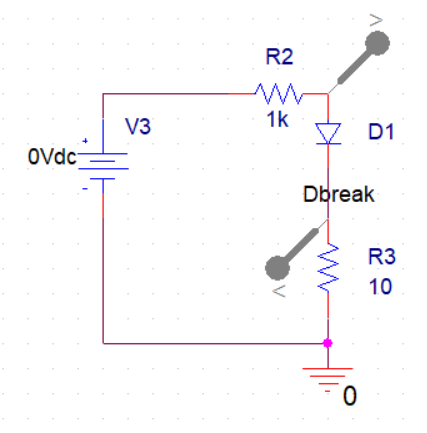
\includegraphics[width = 0.4\textwidth]{Q7/madarAlef.png}}
    \fbox{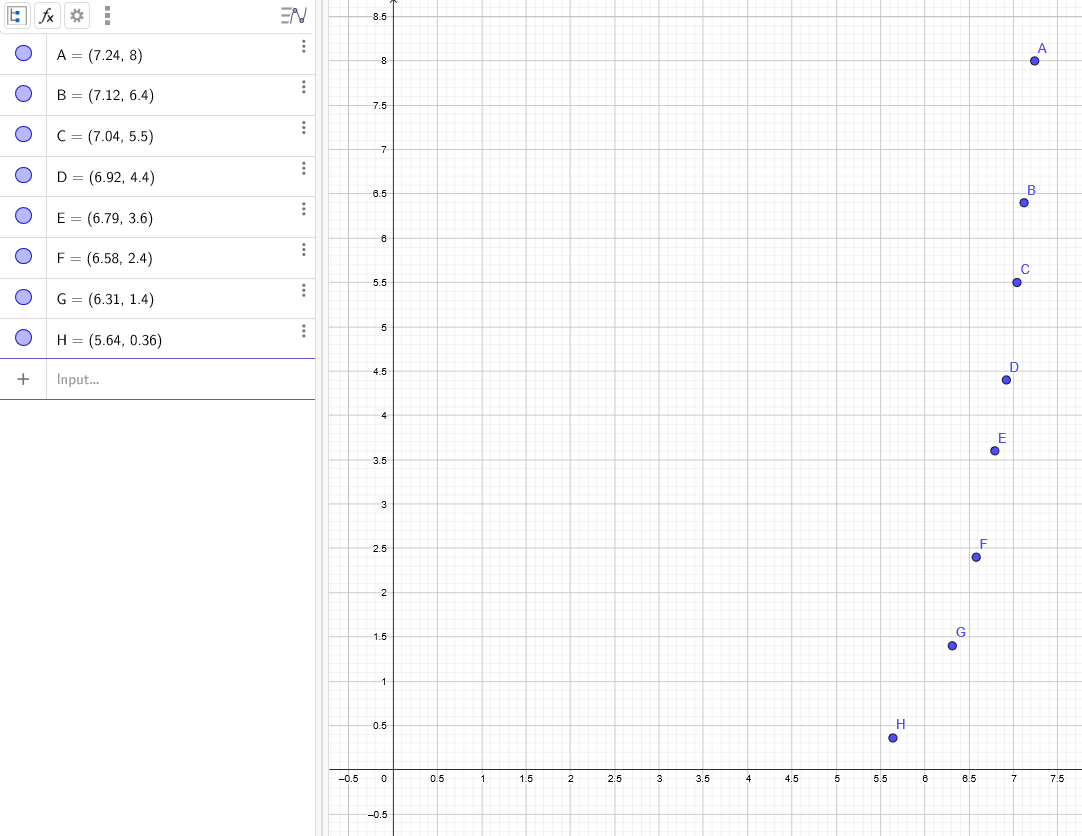
\includegraphics[width = 0.53\textwidth]{Q7/nemudarAlef.png}}
    \caption{مدار بسته شده}
\end{figure}
\begin{latin}
    \begin{table}[h]
        \centering
        \begin{tabular}{|c|c|c|c|c|c|c|c|c|}
            \hline
            V(mV) & 724 & 712 & 704 & 692 & 679 & 658 & 631 & 564  \\
            \hline
            I(mA) & 8   & 6.4 & 5.5 & 4.4 & 3.6 & 2.4 & 1.4 & 0.36 \\
            \hline
        \end{tabular}
        \caption{measured values}
    \end{table}
\end{latin}
که مورد انتظارمان از پیش کزارش بدست آمده است. و مانند به تئوری.\\
\pagebreak
\subsection{ب)}
\begin{figure}[h]
    \centering
    \fbox{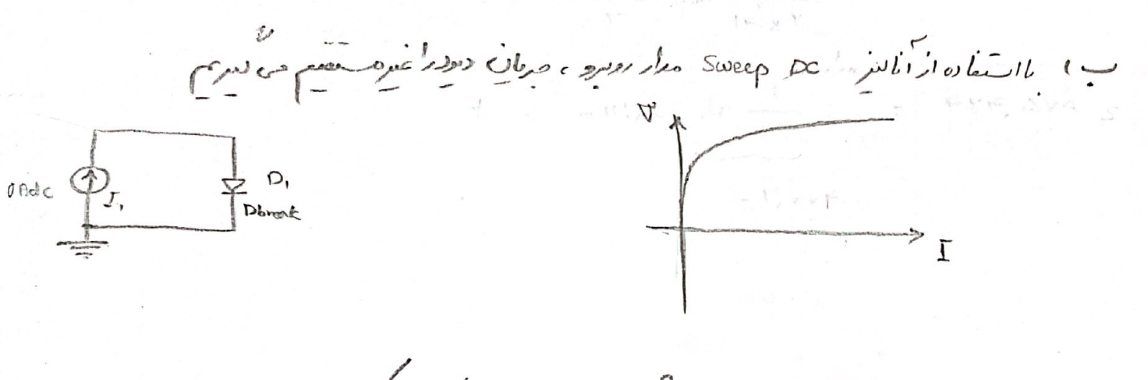
\includegraphics[width = \textwidth]{Q7/pishB.png}}
    \caption{\textcolor{blue}{از پیش گزارش داریم}}
\end{figure}
هم طبق پیش گزارش پیش بینی هایی داریم در مورد نمودار و هم در آزمایش به این
نتیجه میرسیم.\\
مدار طراحی شده مانند مدار قسمت قبل بوده و ما ولتاژ مقاومت را به ورودی
x در اوسیلوسکوپ میدهیم و ولتاژ دیود را به ورودی y میدهیم.\\
حال در صفحه یک نقطه میبینیم که با تکان دادن ولتاژ تکان میخورد.\\
برای این که تمام نمودار را ببینیم ما ولتاژ ورودی را در حالت AC با
فرکانس بالا قرار میدهیم و حالا به طور کامل میبینیم نمودار را.
\begin{figure}[!h]
    \centering
    \fbox{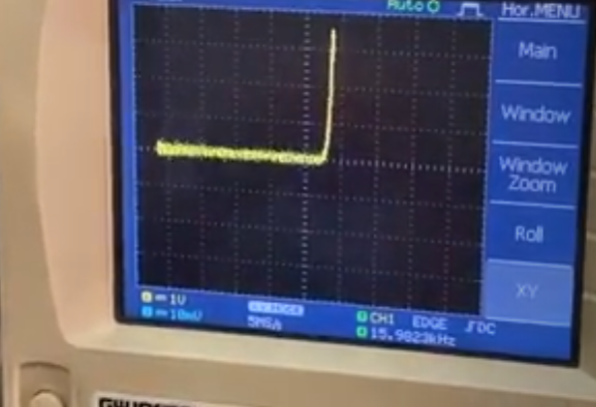
\includegraphics[width = 0.7\textwidth]{Q7/oscB.png}}
    \caption{عکس گرفته شده در آزمایشگاه}
\end{figure}
عکس بدست آمده کاملا مطابق با انتظارمان از تئوری بوده و مشاهده میکنیم که
حدودا در $V=0.7v$ شکست برای دیود رخ میدهد.
\pagebreak
\subsection{ج)}
\begin{figure}[h]
    \centering
    \fbox{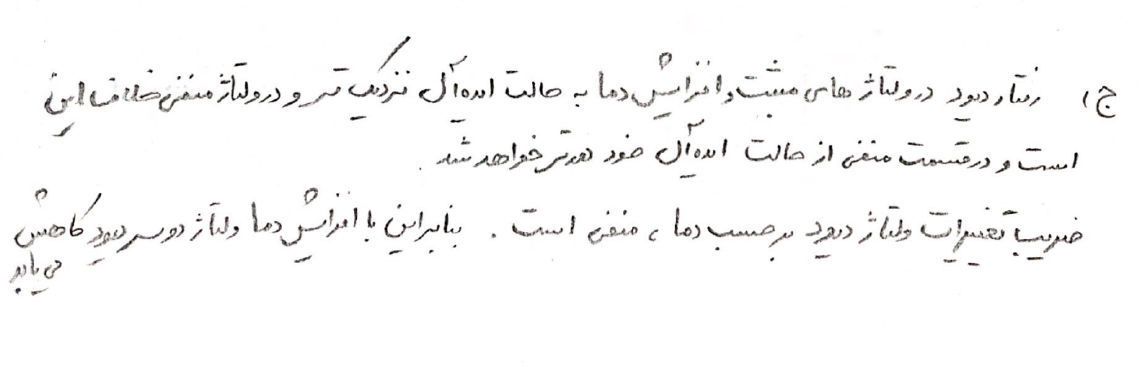
\includegraphics[width = \textwidth]{Q7/pishJ.png}}
    \caption{\textcolor{blue}{از پیش گزارش داریم}}
\end{figure}
این مد مولتی متر به ما ولتاژ شکست را میدهد. \\
دقیقا طبق پیش گزارش در آزمایشگاه مشاهده میکنیم که ولتاژ در حال کاهش است.
\subsubsection{تئوری}
$$I_d = I_0(e^{(\frac{eV}{k_BT})}-1)$$
\pagebreak
